\chapter{Transport Methods}
\label{chapter-methods}

As described perviously, ADIOS provides a framework for the development and
deployment of new techniques for data movement through the use of {\em
  Transport Methods}. While the development of transport is not in the scope of
this manual, the user is given the option to easily select a specific method for
the needs of an application at run time. 

ADIOS includes two broad classes of transport method, mainline methods and
experimental methods. Mainline methods are supported methods that provide both
high performance, reliability and usability. Experimental methods are
under-development research techniques to explore new I/O techniques. While we
encourage our users to experiment with all available methods, no explicit
support is provided for these research methods. 

The \verb+adios_config+ tool lists the transport (write) methods when using the -m option.

\begin{lstlisting}
$ adios_config -m
...
available write methods (in XML <method> element or in adios_select_method()):
    "MPI"
    "POSIX"
    "DATASPACES"
    "PHDF5"
    "MPI_LUSTRE"
    "POSIX1"
    "NC4"
    "MPI_AGGREGATE"
    "FLEXPATH"
    "VAR_MERGE"
...
\end{lstlisting}


%% Because of the time it can take to move data from one process to another or to 
%% write and read data to and from a disk, it is often advantageous to arrange the 
%% program so that some work can be done while the messages are in transit. So far, 
%% we have used non-blocking operations to avoid waiting. Here we describe some details 
%% for arranging a program so that computation and I/O can take place simultaneously.

\section{Mainline Transport Methods}

\subsection{NULL}

The ADIOS NULL method allows users to quickly comment out an ADIOS group by changing 
the transport method to ``NULL,'' users can test the speed of the routine by timing 
the output against no I/O. This is especially useful when working with asynchronous 
methods, which take an indeterminate amount of time.  Another useful feature of 
this I/O is that it quickly allows users to test out the system and determine whether 
bugs are caused by the I/O system or by other places in the codes.

\subsection{POSIX}

The simplest method provided in ADIOS just does binary POSIX I/O operations. Currently, 
it does not support shared file writing or reading and has limited additional functionality. 
The main purpose for the POSIX I/O method is to provide a simple way to migrate 
a one-file-per-process I/O routine to ADIOS and to test the results without introducing 
any complexity from MPI-IO or other I/O methods. Performance gains just by using 
this transport method are likely due to our aggressive buffering for better streaming 
performance to storage. The buffering method writes out files in BP format, which 
is a compact, self-describing format. 

Additional features may be added to the ADIOS POSIX transport method over time. 
A new transport method with a related name, such as POSIX-ASCII, may be provided 
to perform I/O with additional features. The POSIX-ASCII example would write out 
a text version of the data formatted nicely according to some parameters provided 
in the XML file.

\subsection{MPI}

Many large-scale scientific simulations generate a large amount of data, spanning 
thousands of files or datasets. The use of MPI-IO reduces the amount of files and 
thus is helpful for data management, storage, and access. 

The original MPI method was developed based on our experiments with generating 
the better MPI-IO performance on the ORNL Jaguar machine. Many of the insights 
have helped us achieve excellent performance on both the Jaguar XT4 machine and 
on the other clusters. Some of the key insights we have taken advantage of include 
artificially serialized MPI\_File\_open calls and additional timing delays that 
can achieve reduced delays due to metadata server (MDS) conflicts on the attached 
Lustre storage system.

The adapted code takes full advantage of NxM grouping through the coordination-communicator. 
This grouping generates one file per coordination-communicator with the data stored 
sequentially based on the process rank within the communicator.  Figure~\ref{fig:serialized-open} presents 
in the example of GTC code, 32 processes in the same Toroidal zone write to one 
integrated file. Additional serialization of the MPI\_File\_open calls is done 
using this communicator as well because each process may have a different size 
data payload. Rank 0 calculates the size that it will write, calls MPI\_File\_open, 
and then sends its size to rank 1. Rank 1 listens for the offset to start from, 
adds its calculated size, does an MPI\_File\_open, and sends the new offset to 
rank 2. This continues for all processes within the communicator. Additional delays 
for performance based on the number of processes in the communicator and the projected 
load on the Lustre MDS can be used to introduce some additional artificial delays 
that ultimately reduce the amount of time the MPI\_File\_open calls take by reducing 
the bottleneck at the MDS. An important fact to be noted is that individual file 
pointers are retrieved by MPI\_File\_open so that each process has its own file 
pointer for file seek and other I/O operations.

\begin{figure}[htbp]
\begin{center}
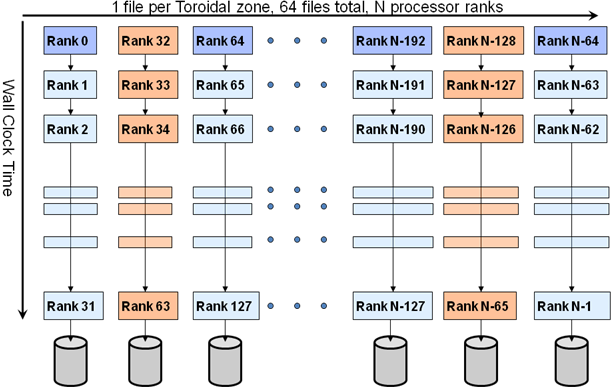
\includegraphics[width=290pt, height=185pt]{figures/mpi-method-serialized-opens.png}
\caption{Server-friendly metadata approach: offset the create/open in time}
\label{fig:serialized-open}
\end{center}
\end{figure}

We built the MPI transport method, mainly with Lustre in mind because it has been 
the primary parallel storage service we have available. However, other file-system-specific 
tunings are certainly possible and fully planned as part of this transport method 
system. For each new file system we encounter, a new transport method implementation 
tuned for that file system, and potentially that platform, can be developed without 
impacting any of the scientific code.

The MPI transport method is the most mature, fully featured, and well tested method 
in ADIOS. We recommend to anyone creating a new transport method that they study 
it as a model of full functionality and some of the advantages that can be made 
through careful management of the storage resources.

\subsection{MPI\_LUSTRE}

The MPI\_LUSTRE method is the MPI method with stripe alignment to achieve even 
greater write performance on the Lustre file system. Each writing process' data 
is aligned to Lustre stripes. This results in better parallelization of the storage 
elements. The drawback of using this method is that empty chunks are created between 
the data sets of the separate processes in the output file, and thus the file size 
is larger than with using the MPI method. The size of an empty space is the difference 
between the size of the output data of one writing process and the total size of 
Lustre stripes that can hold that amount of data, so that the next writing process' 
output starts aligned with another stripe. Choose the stripe size for the output 
file therefore carefully, to make the empty space as small as possible. 

The following XML snippet shows how to use the MPI\_LUSTRE method in ADIOS. 
\begin{lstlisting}[language=XML]
<method group="temperature" method="MPI_LUSTRE">
	stripe_count=16,stripe_size=4194304,block_size=4194304 
</method>
\end{lstlisting}

There are three key parameters used in this method.
\begin{itemize}
\item \textbf{stripe\_count} specifies how many storage targets to 
use for the whole output file. If not set, the default value is 4.

\item \textbf{stripe\_size}  specifies Lustre stripe size in bytes. 
If not set, the default value is 1048576 (i.e. 1 MB).

\item \textbf{block\_size}   specifies the size of each I/O write 
request. As an example, if total data size to be written from one process is 800 
MB at a time, and you want ADIOS to issue twenty I/O write requests issued from 
one process to Lustre during the writing, then the block\_size should be 40MB.
\end{itemize}

Note in 1.3 and later releases, with Lustreapi option enabled in configuration, 
MPI\_LUSTRE sets the parameters automatically and therefore parameters in XML are 
not required.  The method automatically calculates the data size from each processor 
and sets the proper striping parameters. 

\subsection{MPI\_AGGREGATE}
\label{section-method-mpiamr}

The MPI\_AGGREGATE method is designed to maximize write performance for large scale
applications (more than 10,000 cores) that write out data from a large subset of
processors. 
%such as adaptive mesh refinement (AMR) on the Lustre file system. 
%In AMR-like applications, 
%each processor outputs varying amount of data and some can output very small size 
%data. 
Based upon MPI\_LUSTRE method, MPI\_AGGREGATE further improves the write speed by 

\begin{enumerate}
\item aggregating data from multiple MPI processors into large chunks. This effectively 
increases the size of each request and reduces the number of I/O requests.
\item threading the metadata operations such as file open. Users are encouraged to 
call adios\_open and adios\_group\_size API as early as possible. In case Lustre 
MDS has a performance hit, the overall metadata performance won't be affected. 
The following code snippet shows a typical way of using this method to improve 
metadata performance.
\begin{lstlisting}[language=XML]
adios_open(...); 
adios_group_size(...);
...... 
//do your computation
...... adios_write(..); 
adios_write(..); 
adios_close(..);
\end{lstlisting}

\item further removing communication and wide striping overhead by writing out subfiles. 
Please refer to POSIX method on how to read data from subfiles.
\end{enumerate}

The following XML snippet shows how to use MPI\_AGGREGATE method in ADIOS.

There are two key parameters used in this method.

\begin{lstlisting}[language=XML]
<method group="tracers" method="MPI_AGGREGATE"> 
	num_aggregators=24;num_ost=672
</method>
\end{lstlisting}

\begin{itemize}
\item \textbf{num\_aggregators} specifies the number of aggregators 
to use.
\item \textbf{num\_ost }specifies the number of Lustre storage targets 
 available in the file system. Note this parameter is mandatory if ``---with-lustre'' 
option is not given during ADIOS configuration.
\end{itemize}

For example, if you have an MPI job with 120,000 processors and the number of aggregator 
is set to 2400, then each aggregator will aggregate the data from 120,000/2400=50 
processors.

The MPI\_AGGREGATE method allocates stand-alone internal buffers for aggregating data. 
As opposed to ADIOS buffer (the size of which is set from XML file), these buffers 
are allocated separately and the total size (on one processor) is twice the ADIOS 
group size. User needs to make sure each process has enough memory when using this 
method.  

Note that in 1.3 and later releases, with Lustreapi option enabled in configuration, 
MPI\_AGGREGATE sets the parameters automatically and therefore parameters in XML are 
not required. The method automatically calculates the data size from each processor 
and sets the proper aggregation parameters. Also note that in previous versions
of ADIOS (before 1.4), the MPI\_AGGREGATE method was refered to as the MPI\_AMR
method. 


\subsection{VAR\_MERGE}
\label{section-method-varmerge}
The VAR\_MREGE method is designed to extends the capability of current ADIOS
methods to address the I/O challenges for applications
that write out small variables at scale. During data output, 
VAR\_MERGE merges the small variable blocks from intensive chunking into
larger data chunks with their spatial localities are reserved. The benefits
are: 1) less contention at storage side during data
output; 2) frequent read and seek operations can be avoided during reading.
An example of variable merging is given in Figure~\ref{fig:sar}. 


\begin{figure}[htbp]
\begin{center}
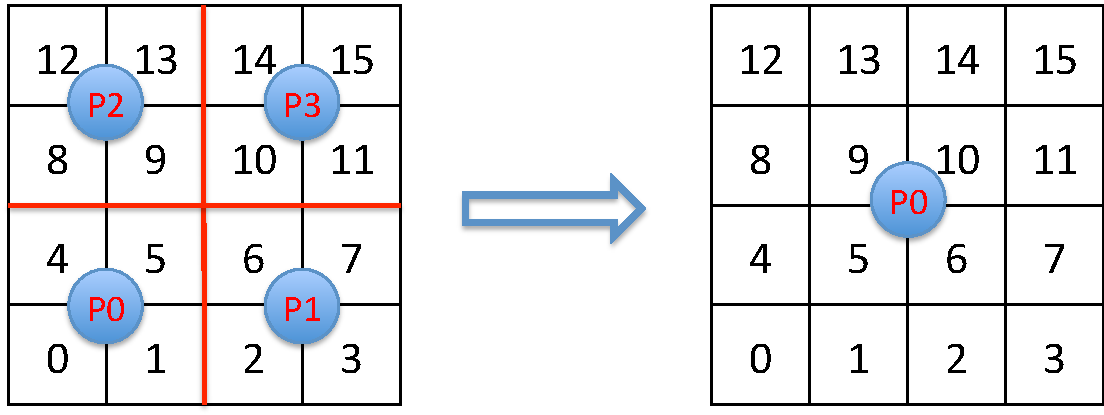
\includegraphics[width=0.5\columnwidth]{figures/sar.pdf}
\caption{Spatial Aggregation of a 4x4 2D Variable From 4 proceeses to Process 0}
\label{fig:sar}
\end{center}
\end{figure}


The following XML snippet shows how to use VAR\_MERGE method in ADIOS.
There are two key parameters used in this method.

\begin{lstlisting}[language=XML]
<method group="test" method="VAR_MERGE"> chunk_size=2097152; io_method=MPI_AGGREGATE; 
    io_parameters=num_aggregators=24,num_ost=672
</method>
\end{lstlisting}

\begin{itemize}
\item \textbf{chunk\_size} specifies the chunk size after merging. If
merging current data chunk leads to a chunk size that is larger than this
value, merging will not be performed. The default value is 2MB without  
specification in XML.  

\item \textbf{io\_method} the underlying I/O method for data output.  
The ADIOS transport method that VAR\_MERGE can work with include POSIX, MPI,
    MPI\_LUSTRE and MPI\_AGGREGATE. 

\item \textbf{io\_parameters} the parameters required for using the
io\_method. Note that the paramters needs to be separated by ",".  
\end{itemize}

For example, if you want to merge data chunks into 4MB chunks and use
MPI\_LUSTRE method to write out data, your XML looks like:  

\begin{lstlisting}[language=XML]
<method group="test" method="VAR_MERGE"> chunk_size=4194304,
    io_method=MPI_LUSTRE, io_parameters=stripe_count=128,stripe_size=4194304
</method>
\end{lstlisting}

Here we specified the data to be placed on 128 storage targes, and the stripe
size is 4MB.
Note that current VAR\_MERGE method only supports 1D, 2D and 3D variables.
The maximum level of aggregation is 2 due to the consideration of
merging overhead.  

\subsection{Dataspaces}
\label{section-method-dataspaces}

Dataspaces is an asynchronous I/O transfer method within ADIOS that enables low-overhead, 
high-throughput data extraction from a running simulation. Dataspaces consists of two 
main components: (1) a client module using the ADIOS Dataspaces method, and (2)
a dataspaces\_server module. Internally, 
Dataspaces uses RDMA to implement the communication, coordination, and data transport 
between the clients and the dataspaces\_server modules.

The dataspaces clients use a light-weight library that provides the asynchronous
I/O API to be used by ADIOS. It is integrated with the ADIOS layer and the
functionality is exposed through the ADIOS write/read semantics. 
%It integrates with the ADIOS layer by extending the generic ADIOS data transport 
%hooks. 
The ADIOS layer is used to collect and encode the data written 
by the application into a local transport buffer. Once it has collected data from 
an application, the transport method notifies the dataspaces\_server through a coordination channel 
that it has data available to send out. At this point, the control is
transferred back to the application, while the data is asynchronously extracted 
by the dataspaces\_server.

The dataspaces\_server module is a stand-alone service that runs independently of a simulation 
on a set of dedicated nodes in the 
{\em staging area}. It transfers data from the application through RDMA,  
and can save it to local storage system, e.g., the Lustre file system, stream it to 
remote sites, e.g., auxilliary clusters, or serve it directly from the staging area to 
other applications. One instance of the dataspaces\_server can service multiple applications 
 in parallel. Further, the server can run in cooperative mode (i.e., multiple 
instances of the server cooperate to service the application in parallel and to balance 
load). The dataspaces\_server receives notification messages from the transport method, schedules 
the requests, and initiates the data transfers  in parallel. The 
server schedules and prioritizes the data transfers while the simulation is computing 
in order to overlap data transfers with computations, to maximize data throughput, 
and to minimize the overhead on the application.

Dataspaces is an asynchronous method available in ADIOS, that can be selected by specifying 
the transport method in the external ADIOS XML configuration file as ``Dataspaces''.

\begin{lstlisting}[language=XML, caption=Select Dataspaces as a transport method in the configuration file example.]
<method group="fluxdiag" method="Dataspaces"/>
\end{lstlisting}

To make use of the Dataspaces transport, an application job needs to also run the dataspaces\_server 
component together with the application. The server should be configured and started 
before the application as a separate job in the system. For example:

\begin{lstlisting}[language=bash, caption=Start the server component in a job file first.]
aprun -n $SPROC ./dataspaces_server -s $SPROC -c $PROC &> log.server &
\end{lstlisting}

The variable \$SPROC represents the number of server instances to run, and the 
variable \$PROC represents the number of application processes. For example if 
the job script runs a coupling scenario with two applications that run on 128 and 
432 processors respectively, then the value of \$PROC is 560. The `\&' character 
at the end of the line would place the `aprun' command in the background, and will 
allow the job script to continue and run the other applications. The server processes 
produce a configuration file, i.e., `conf' that is used by the application  
to connect to the servers. This file contains identifying information of the 
master server, which coordinates the client registration 
and discovery process. The job script should wait for the servers to start-up and 
produce the `conf' file before starting the client application processes. 
%, which it can then export to environment variables, e.g., 
%P2TNID, and P2TPID. 
Once ADIOS is initialized in the application, this configuration file is parsed
to provide the rendevouz information. 

\begin{lstlisting}[language=C, caption=Wait for server start-up completion and export the configuration to environment variables.]
while [ ! -f conf ]; do
	echo "Waiting for servers to start-up"
	sleep 2s
done


while read line; do
	export set "${line}"
done < conf
\end{lstlisting}

The server component will terminate automatically when the applications finish. 
The clients  will send an unregister message to the server before 
they finish execution, and the servers will exit after they receive \$PROC unregister 
messages.

%% The Dataspaces transport method is experimental and is not included with the public version 
%% of the ADIOS source code in this release; however it is available for use on the 
%% XT4 and XT5 machines at ORNL.

\subsection{DIMES}
\label{section-method-dimes}
% DIstributed MEmory Space (DIMES)
DIMES is another asynchronous I/O transfer method within ADIOS that enables low-
latency, scalable data extraction from a running simulation. It is designed to enable M$
\times$N parallel data redistribution between tightly coupled applications, which 
essentially performs RDMA-based memory-to-memory transfers of distributed data such 
as global arrays from M processes of one application to N processes of another application.

Both DIMES and Dataspaces methods are implemented based upon the open source 
software library DataSpaces. However, unlike Dataspaces method which implements 
memory-to-memory data sharing using dedicated server nodes in the \emph{staging 
area}, DIMES method implements the parallel data redistribution through point-to-point 
transfers directly between processes of data writing and reading applications, and thus 
bypass the \emph{staging area}. 

For applications using the ADIOS DIMES method, the new functionality is exposed 
through the ADIOS write/read semantics. ADIOS layer is used to collect data written by 
the application into a local RDMA memory buffer as data objects that can 
be remotely accessed through the underlying RDMA get operations. Once data is 
successfully copied from the application space, the control is transferred back to the 
application, then the simulation data can be asynchronously extracted and redistributed 
to the coupled reading applications. 

Though the DIMES methods does not need simulation data to be transferred to the 
\emph{staging area}, a stand-alone server module is still required for constructing a 
distributed directory service to keep track of the in-memory data objects. Internally, client 
applications would query the service to locate required data objects, and then perform 
the subsequent RDMA-based parallel data transfers. 

DIMES method can be selected by specifying the transport method in the external 
ADIOS XML configuration file (as below).

\begin{lstlisting}[language=XML, caption=Select DIMES as a transport method in the configuration file example.]
<method group="fluxdiag" method="DIMES"/>
\end{lstlisting}

The dataspaces\_server component is extended to support the data locating service 
mentioned above. To make use of the DIMES method, a job needs to also run the 
dataspaces\_server with the applications. Each dataspaces\_server instance 
needs to run on one dedicated processor core, and multiple sever instances can be 
started in parallel to support the data locating service for larger scale applications. 
Instructions on how to configure and run the dataspaces\_server can be found in 
section~\ref{section-method-dataspaces}.


\subsection{Flexpath}
\label{section-method-flexpath}
Flexpath is an asynchronous data transport method built to ensure scalable I/O through the use of staging areas. It is built on top of the EVPath event-driven messaging library \url{http://www.cc.gatech.edu/systems/projects/EVPath/}, which allows for the creation of arbitrary network overlays. Data sent through EVPath is serialized with the Fast, Flexible Serialization (FFS) library, and also allows for additional metadata to be appended to the datastream through the use of separately addressable attributes. To provide high-performance, Flexpath takes advantage of EVPath features such as {\em multiqueue stones} and {\em C-on-Demand (COD)} dynamic code generation.

Flexpath also works on top of several popular high-end network interfaces, such as Infiniband, Portals, and Gemini. See the intallation section for information on how to use this functionality. 


\subsection{PHDF5}

HDF5, as a hierarchical File structure, has been widely adopted for data storage 
in various scientific research fields.  Parallel HDF5 (PHDF5) provides a series 
of APIs to perform the I/O operations in parallel from multiple processors, which 
dramatically improves the I/O performance of the sequential approach to read/write 
an HDF5 file. In order to make the difference in transport methods and file formats 
transparent to the end users, we provide a mechanism that write/read an HDF5 file 
with the same schema by keeping the same common adios routines with only one entry 
change in the XML file. This method provides users with the capability to write 
out exactly the same HDF5 files as those generated by their original PHDF5 routines. 
Doing so allows for the same analysis tool chain to analyze the data. 

Currently, HDF5 supports two I/O modes: independent and Collective read or write, 
which can use either the MPI or the POSIX driver by specifying the dataset transfer 
property list in H5Dwrite function calls. In this release, only the MPI driver 
is supported in ADIOS.
This requires that every process participates in the writing of each variable. 

Note: Do not expect better performance with ADIOS/PHDF5 than with PHDF5 itself. ADIOS does not write differently to a HDF5 formatted file, it simply uses PHDF5 function calls to write out data. 

%later on, both I/O drivers will be supported by changing 
%the attribute information for PHDF5 method elements in XML. 

\subsection{NetCDF4}

Another widely accepted standard file format is NetCDF, which is the most frequently 
used file format in the climate and weather research communities.  Beginning with 
the NetCDF 4.0 release, NetCDF has added PHDF5 as a new option for data storage 
called the ``netcdf-4 format''.  When a NetCDF4 file is opened in this new format, 
NetCDF4 inherits PHDF5's parallel I/O capabilities.

The NetCDF4 method creates a single shared filed in the ``netcdf-4 format'' and 
uses the parallel I/O features.  The NetCDF4 method supports multiple open files. 
 To select the NetCDF4 method use ``NC4'' as the method name in the XML file.

\textbf{Restrictions:} Due to the collective nature of the NetCDF4 API, there are 
some legal XML files that will not work with the NetCDF4 method.  The most notable 
incompatibility is an XML fragment that creates an array variable without a surrounding 
global-bounds.  Within the application, a call to adios\_set\_path() is used to 
add a unique prefix to the variable name.  A rank-based prefix is an example. 

\begin{lstlisting}[language=XML, caption=Example XML]
<?xml version="1.0"?> 
<adios-config host-language="C">
	<adios-group name="atoms " coordination-communicator="comm"> 
		<var name="nparam" type="integer"/>
		<var name="ntracked" type="integer"/>
		<var name="atoms " type="real" dimensions="nparam,ntracked"/> 
	</adios-group>
	<method group="atoms" method="NC4"/> 
	<buffer size-MB="1" allocate-time="now"/> 
</adios-config>
\end{lstlisting}

\begin{lstlisting}[language=C, caption=Example C source]
char path[1024];
adios_init ("config.xml", comm);
adios_open (&adios_handle, "atoms", filename, "w", comm); 
sprintf(path, "node_%d_", myrank); 
adios_set_path(adios_handle, path);
#include "gwrite_atoms.ch" 
adios_close (adios_handle); 
adios_finalize (myrank);
\end{lstlisting}

This technique is an optimization that allows each rank to creates a variable of 
the exact dimensions of the data being written.  In this example, each rank may 
be tracking a different number of atoms.

The NetCDF4 collective API expects each rank to write the same variable with the 
same dimensions.  The example violates both of these expectations.

Note: NetCDF4 files created in the new ``netcdf-4 format'' cannot be opened with 
existing tools linked with NetCDF 3.x.  However, NetCDF4 provides a backward compatibility 
API, so that these tools can be relinked with NetCDF4.  After relink, these tools 
can open files in the ``netcdf-4 format''.


\section{Research Methods}

ADIOS provides an easy plug-in mechanism for users or developers to design their 
own transport method. A step-by-step instruction for inserting a new I/O method 
is given in the Developer's manual. Users are likely to choose the best method from among 
the supported or customized methods for the running their platforms, thus avoiding 
the need to verify their source codes due to the switching of I/O methods.

%% \section{Asynchronous methods}

\subsection{Network Scalable Service Interface (NSSI)}

The Network Scalable Service Interface (NSSI) is a client-server development framework 
for large-scale HPC systems.  NSSI was originally developed out of necessity for 
the Lightweight File Systems (LWFS) project, a joint effort between researchers 
at Sandia National Laboratories and the University of New Mexico.  The LWFS approach 
was to provide a core set of fundamental capabilities for security, data-movement, 
and storage, and allow extensibility through the development of additional services. 
 The NSSI framework was designed to be the vehicle to enable the rapid development 
of such services.

The NSSI method is composed of two components - a client method and a staging service. 
 The client method does not perform any file I/O.  Instead, all ADIOS operations 
become requests to the staging service.  The staging service is an ADIOS application, 
which allows the user to select any ADIOS method for output.  Client requests fall 
into two categories - pass-through and cached.  Pass-through requests are requests 
that are synchronous on the staging service and return an error immediately on 
failure.  adios\_open() is an example of a pass-through request.  Cached requests 
are requests that are asynchronous on the staging service and return an error at 
a later time on failure.  adios\_write() is an example of a cached request.  All 
data cached for a particular file is aggregated and flushed when the client calls 
adios\_close().

Each component requires its own XML config file.  The client method can be selected 
in the client XML config using ``NSSI'' as the method.  The service XML config 
must be the same as the client XML config except that the method is ``NSSI\_FILTER''. 
 When the NSSI\_FILTER method is selected, the ``submethod'' parameter is required. 
 The ``submethod'' parameter specifies the ADIOS method that the staging service 
will use for output.  Converting an existing XML config file for use with NSSI 
is illustrated in the following three Figures.

\begin{lstlisting}[language=XML, caption=Example Original Client XML]
<method method="MPI" group="atoms">max_storage_targets=160</method>
\end{lstlisting}

\begin{lstlisting}[language=XML, caption=Example NSSI Client XML]
<method method="NSSI" group="atoms"/>
\end{lstlisting}

\begin{lstlisting}[language=XML, caption=Example NSSI Staging Service XML]
<method method="NSSI_FILTER" group="atoms"> 
	submethod="MPI" ;subparameters="max_storage_targets=160"
</method>
\end{lstlisting}

After creating new config files, the application's PBS script (or other runtime 
script) must be modified to start the staging service prior to application launch 
and stop the staging service after application termination. The ADIOS distribution 
includes three scripts to help with these tasks.

The start.nssi.staging.sh script launches the staging service.  start.nssi.staging.sh 
takes two arguments - the number of staging services and an XML config file.

The create.nssi.config.sh script creates an XML file that the NSSI method uses 
to locate the staging services.  create.nssi.config.sh takes two arguments - the 
name of the output config file and the name of the file containing a list of service 
contact info.  The service contact file is created by the staging service at startup. 
 The staging service uses the ADIOS\_NSSI\_CONTACT\_INFO environment variable to 
determine the pathname of the contact file.

The kill.nssi.staging.sh script sends a kill request to the staging service.  kill.nssi.staging.sh 
 takes one argument - the name of the file containing a list of service contact 
info (ADIOS\_NSSI\_CONTACT\_INFO).  The staging service will gracefully terminate.

\begin{lstlisting}[language=bash, caption={Example PBS script with NSSI Staging Service}, label=list-nssi-pbs-script]
#!/bin/bash
#PBS -l walltime=01:00:00,size=128

export RUNTIME_PATH=/tmp/work/$USER/genarray3d.$PBS_JOBID
mkdir -p $RUNTIME_PATH
cd $RUNTIME_PATH


export ADIOS_NSSI_CONTACT_INFO=$RUNTIME_PATH/nssi_contact.xml
export ADIOS_NSSI_CONFIG_FILE=$RUNTIME_PATH/nssi_config.xml 
$ADIOS_DIR/scripts/start.nssi.staging.sh 4 \
	$RUNTIME_PATH/genarray3d.server.xml >server.log 2>&1 &
sleep 3
$ADIOS_DIR/scripts/create.nssi.config.sh \
	$ADIOS_NSSI_CONFIG_FILE $ADIOS_NSSI_CONTACT_INFO 

aprun -n 64 $ADIOS_SRC_PATH/tests/genarray/genarray \
	$RUNTIME_PATH/test.output 4 4 4 128 128 80 >runlog 

$ADIOS_DIR/scripts/kill.nssi.staging.sh $ADIOS_NSSI_CONTACT_INFO
\end{lstlisting}

Listing~\ref{list-nssi-pbs-script} is a example PBS script that highlights the changes required to launch 
the NSSI staging service.

\textbf{Required Environment Variables.}  The NSSI Staging Service requires that 
the ADIOS\_NSSI\_CONTACT\_INFO variable be set.  This variable specifies the full 
pathname of the file that the service uses to save its contact information.  Depending 
on the platform, the contact information is a NID/PID pair or a hostname/port pair. 
 Rank0 is responsible for gathering the contact information from all members of 
the job and writing the contact file.  The NSSI method requires that the ADIOS\_NSSI\_CONFIG\_FILE 
variable be set.  This variable specifies the full pathname of the file that contains 
the complete configuration information for the NSSI method.  A configuration file 
with contact information and reasonable defaults for everything else can be created 
with the create.nssi.config.sh script.

\textbf{Calculating the Number of Staging Services Required.}  Remember that all 
adios\_write() operations are cached requests.  This implies that the staging service 
must have enough RAM available to cache all data written by its clients between 
adios\_open() and adios\_close().  The current aggregation algorithm requires a 
buffer equal to the size of the data into which the data is aggregated.  The start.nssi.staging.sh 
script launches a single service per node, so the largest amount of data that can 
be cached per service is 50\% of the memory on a node minus system overhead.  System 
overhead can be estimated at 500MB.  If a node has 16GB of memory, the amount of 
data that can be cached is 7.75GB ((16GB-500MB)/2).  To balance the load on the 
staging services, the number of clients should be evenly divisible by the number 
of staging services.

\textbf{Calculating the Number of Additional Cores Required for Staging.}  The 
NSSI staging services run on compute nodes, so additional resources are required 
to run the job.  For each staging service required, add the number of cores per 
node to the size of the job.  If each node has 12 cores and the job requires 16 
staging services, add 192 cores to the job.

The NSSI transport method is experimental and is not included with the public version 
of the ADIOS source code in this release; however it is available for use on the 
XT4 and XT5 machines at ORNL.

\subsection{DataTap}

DataTap is an asynchronous data transport method built to ensure very high levels 
of scalability through server-directed I/O. It is implemented as a request-read 
service designed to bridge the order-of-magnitude difference between available 
memories on the I/O partition compared with the compute partition. We assume the 
existence of a large number of compute nodes producing data (we refer to them as 
``\textit{DataTap }clients'') and a smaller number of I/O nodes receiving the data 
(we refer to them as ``\textit{DataTap }servers'') (see Figure~\ref{fig:datatap-arch}). 

\begin{figure}[htbp]
\begin{center}
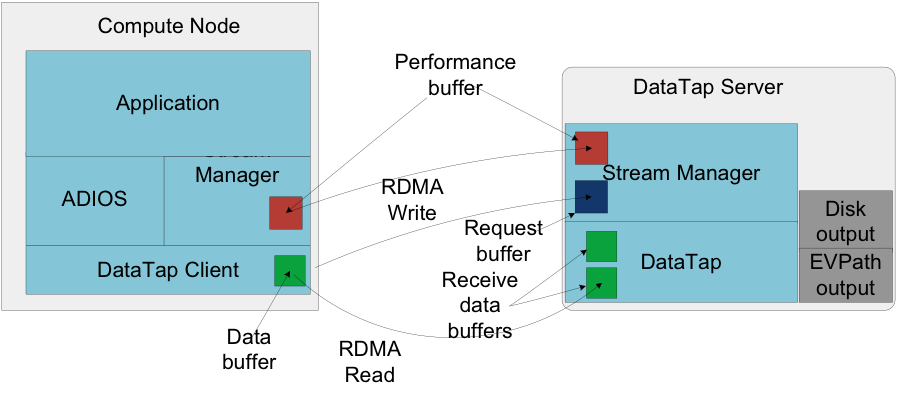
\includegraphics[width=222pt, height=97pt]{figures/datatap-architecture.png}
\caption{DataTap architecture}
\label{fig:datatap-arch}
\end{center}
\end{figure}


Upon application request, the compute node marks up the data in PBIO format and 
issues a request for a data transfer to the server. The server queues the request 
until sufficient receive buffer space is available. The major cost associated with 
setting up the transfer is the cost of allocating the data buffer and copying the 
data. However, this overhead is small enough to have little impact on the overall 
application runtime. When the server has sufficient buffer space, a remote direct 
memory access (RDMA) read request is issued to the client to read the remote data 
into a local buffer. The data are then written out to disk or transmitted over 
the network as input for further processing in the I/O Graph. 

We used the Gyrokinetic Turbulence Code (GTC) as an experimental tested for the 
DataTap transport. GTC is a particle-in-cell code for simulating fusion within 
tokamaks, and it is able to scale to multiple thousands of processors. In its default 
I/O pattern, the dominant I/O cost is from each processor writing out the local 
particle array into a file. Asynchronous I/O reduces this cost to just a local 
memory copy, thereby reducing the overhead of I/O in the application.

The DataTap transport method is experimental and is not included with the public 
version of the ADIOS source code in this release; however it is available for use 
on the XT4 and XT5 machines at ORNL.


%\section{Other research methods at ORNL}

\subsection{MPI-CIO}

MPI-IO defines a set of portable programming interfaces that enable multiple processes 
to have concurrent access to shared files [1]. It is often used to store and retrieve 
structured data in their canonical order. The interfaces are split into two types: 
collective I/O and independent I/O. Collective functions require all processes 
to participate. Independent I/O, in contrast, requires no process synchronization.

Collective I/O enables process collaboration to rearrange I/O requests for better 
performance [2,3]. The collective I/O method in ADIOS first defines MPI fileviews 
for all processes based on the data partitioning information provided in the XML 
configuration file. ADIOS also generates MPI-IO hints, such as data sieving and 
I/O aggregators, based on the access pattern and underlying file system configuration. 
The hints are supplied to the MPI-IO library for further performance enhancement. 
The syntax to describe the data-partitioning pattern in the XML file uses the \texttt{<}global-bounds 
dimensions offsets\texttt{>} tag, which defines the global array size and the offsets 
of local subarrays in the global space. 

The global-bounds element contains one or more nested var elements, each specifying 
a local array that exists within the described dimensions and offset.  Multiple 
global-bounds elements are permitted, and strictly local arrays can be specified 
outside the context of the global-bounds element.

As with other data elements, each of the attributes of the global-bounds element 
is provided by the adios\_write call. The dimensions attribute is specified by 
all participating processes and defines how big the total global space is.  This 
value must agree for all nodes. The offset attribute specifies the offset into 
this global space to which the local values are addressed. The actual size of the 
local element is specified in the nested var element(s).  For example, if the global 
bounds dimension were 50 and the offset were 10, then the var(s) nested within 
the global-bounds would all be declared in a global array of 50 elements with each 
local array starting at an offset of 10 from the start of the array.  If more than 
one var is nested within the global-bounds, they share the declaration of the bounds 
but are treated individually and independently for data storage purposes. 

This research method is installed on Jaguar at ORNL only but is not part of the 
public release.

\subsection{MPI-AIO}

The initial implementation of the asynchronous MPI-IO method (MPI-AIO) is patterned 
after the MPI-IO method. Scheduled metadata commands are performed with the same 
serialization of MPI\_Open calls as given in Figure~\ref{fig:serialized-open}.

The degree of I/O synchronicity depends on several factors. First, the ADIOS library 
must be built with versions of MPI that are built with asynchronous I/O support 
through the MPI\_File\_iwrite, MPI\_File\_iread, and MPI\_Wait calls. If asynchronous 
I/O is not available, the calls revert to synchronous (read blocking) behavior 
identical to the MPI-IO method described in the previous section. 

Another important factor is the amount of available ADIOS buffer space. In the 
MPI-IO method, data are transported and ADIOS buffer allocation is reclaimed for 
subsequent use with calls to adios\_close (). In the MPI-AIO method, the ``close'' 
process can be deferred until buffer allocation is needed for new data. However, 
if the buffer allocation is exceeded, the data must be synchronously transported 
before the application can proceed.

The deferral of data transport is key to effectively scheduling asynchronous I/O 
with a computation. In ADIOS version 1.4, the application explicitly signals that 
data transport must be complete with intelligent placement of the adios\_close 
() call to indicate when I/O must be complete. Later versions of ADIOS will perform 
I/O between adios\_begin\_calculation and adios\_end\_calculation calls, and complete 
I/O on adios\_end\_iteration calls.

This research module is not released in ADIOS 1.4.
